\subsection{Boot Entry Point: MINIX Label to pre\_init()}

\section{Overview}

The MINIX kernel execution begins at the \texttt{MINIX} label in \texttt{head.S}, the
lowest-level assembly code executed after the bootloader transfers control. This chapter
traces every instruction and its effect on CPU state, memory, and control flow.

\section{WHAT: Actions at Entry Point}

\subsection{High-Level Sequence}

At the \texttt{MINIX} label:

\begin{enumerate}
\item \textbf{Jump to multiboot\_init}: Entry point branches immediately
\item \textbf{Set up stack}: Initialize ESP for C execution
\item \textbf{Clear flags}: Set known-good CPU state
\item \textbf{Pass multiboot info}: Push bootloader parameters
\item \textbf{Call pre\_init()}: Transfer to C-level initialization
\end{enumerate}

\section{WHEN: Execution Timing}

\textbf{Time relative to power-on}: $t_0 + \Delta t_{\text{firmware}} + \Delta t_{\text{bootloader}}$

Typical timeline:
\begin{table}[h!]
\centering
\caption{Boot Timeline from Power-On}
\begin{tabular}{lll}
\toprule
Stage & Duration & Cumulative \\
\midrule
BIOS/UEFI & 100-500ms & 100-500ms \\
Bootloader & 50-200ms & 150-700ms \\
Kernel Entry & 0.1-1ms & \textbf{Control reaches MINIX} \\
\bottomrule
\end{tabular}
\end{table}

\what{At the moment execution reaches the MINIX label, the bootloader has already
set up basic hardware: CPU in 32-bit protected mode, A20 gate enabled, GDT loaded,
memory accessible.}

\section{WHY: Architectural Decisions}

\subsection{Entry Point at MINIX Label}

\textbf{Multiboot Specification Compliance}:
The bootloader (GRUB, QEMU, etc.) locates the Multiboot header in the kernel image
and transfers execution to the \texttt{MINIX} label upon matching the magic number.

\why{MINIX uses the Multiboot protocol to support multiple bootloaders without
bootloader-specific code. This abstraction allows MINIX to run on GRUB, QEMU, Xen,
and other Multiboot-compliant platforms with identical kernel code.}

\subsection{Immediate Jump to multiboot\_init}

The first instruction is \texttt{jmp multiboot\_init}---a deliberate control transfer.

\why{This architecture allows the Multiboot header to be located at a fixed offset
in the kernel image (required by the Multiboot spec) while the actual entry code
(\texttt{multiboot\_init}) can be placed elsewhere. The stub at \texttt{MINIX} ensures
the magic number location is correct without constraining code layout.}

\section{HOW: Instruction-Level Execution}

\subsection{Source Code: head.S (Lines 36-77)}

\begin{lstlisting}[style=asmstyle,caption={MINIX Entry Point and Multiboot Header}]
.global MINIX
MINIX:
/* this is the entry point for the MINIX kernel */
    jmp multiboot_init

/* Multiboot header here*/

.balign 8

#define MULTIBOOT_FLAGS (MULTIBOOT_HEADER_WANT_MEMORY |
                        MULTIBOOT_HEADER_MODS_ALIGNED)

multiboot_magic:
    .long MULTIBOOT_HEADER_MAGIC
multiboot_flags:
    .long MULTIBOOT_FLAGS
multiboot_checksum:
    .long -(MULTIBOOT_HEADER_MAGIC + MULTIBOOT_FLAGS)
    .long 0
    .long 0
    .long 0
    .long 0
    .long 0
/* Video mode */
multiboot_mode_type:
    .long MULTIBOOT_VIDEO_MODE_EGA
multiboot_width:
    .long MULTIBOOT_CONSOLE_COLS
multiboot_height:
    .long MULTIBOOT_CONSOLE_LINES
multiboot_depth:
    .long 0

multiboot_init:
    mov    $load_stack_start, %esp    /* make usable stack */
    mov    $0, %ebp
    push   $0                          /* set flags to known good state */
    popf                               /* esp, clear nested task and int enable */
    push   $0

    push   %ebx                        /* multiboot information struct */
    push   %eax                        /* multiboot magic number */
    call   _C_LABEL(pre_init)

    /* Kernel is mapped high now and ready to go, with
     * the boot info pointer returned in %eax.
\end{lstlisting}

\subsection{Instruction-by-Instruction Analysis}

\subsubsection{jmp multiboot\_init (at MINIX label)}

\how{
\begin{enumerate}
\item \textbf{Instruction}: 1-byte opcode (EB xx for short jmp)
\item \textbf{Effect}: Sets EIP = address of multiboot\_init label
\item \textbf{CPU State Change}: EIP register updated
\item \textbf{Timing}: 1-3 CPU cycles (depends on pipeline state)
\item \textbf{Memory Effect}: None; instruction fetch only
\item \textbf{Register State}: All other registers unchanged
\end{enumerate}
}

\subsubsection{mov \$load\_stack\_start, \%esp}

\how{
\begin{enumerate}
\item \textbf{Instruction}: Load immediate 32-bit value into ESP
\item \textbf{Effect}:
  \begin{itemize}
    \item ESP = address of load\_stack\_start (in kernel's BSS section)
    \item Stack pointer is now positioned to grow downward
  \end{itemize}
\item \textbf{CPU State Change}: ESP register updated
\item \textbf{Timing}: 1 CPU cycle (immediate load)
\item \textbf{Register State}:
  \begin{itemize}
    \item Before: ESP has bootloader value (undefined for our purposes)
    \item After: ESP points to known kernel stack location
  \end{itemize}
\end{enumerate}
}

\subsubsection{mov \$0, \%ebp}

\how{
\begin{enumerate}
\item \textbf{Instruction}: Load immediate 0 into EBP
\item \textbf{Effect}: Zero EBP to create known base frame pointer
\item \textbf{Reason}: Prevents stack unwinding tools from walking past boot code
\item \textbf{CPU State Change}: EBP = 0
\item \textbf{Timing}: 1 CPU cycle
\end{enumerate}
}

\subsubsection{push \$0; popf}

\how{
\begin{enumerate}
\item \textbf{Instruction Sequence}:
  \begin{enumerate}
    \item \texttt{push \$0}: Push 0 onto stack
    \item \texttt{popf}: Pop into EFLAGS register
  \end{enumerate}
\item \textbf{Effect}: Sets CPU flags to known state
\begin{itemize}
    \item CF (Carry Flag) = 0
    \item PF (Parity Flag) = 0
    \item AF (Auxiliary Carry) = 0
    \item ZF (Zero Flag) = 0
    \item SF (Sign Flag) = 0
    \item TF (Trap Flag) = 0 (debugging disabled)
    \item IF (Interrupt Flag) = 0 (interrupts disabled during boot)
    \item DF (Direction Flag) = 0 (string ops forward)
    \item OF (Overflow Flag) = 0
\end{itemize}
\item \textbf{Why}: Ensures deterministic C code execution
\item \textbf{Timing}: 2 CPU cycles
\item \textbf{ESP Effect}: ESP += 4 after pop (stack restored)
\end{enumerate}
}

\subsubsection{push \%ebx; push \%eax}

\how{
\begin{enumerate}
\item \textbf{Instruction Sequence}:
  \begin{enumerate}
    \item \texttt{push \%ebx}: Push bootloader-provided Multiboot info structure address
    \item \texttt{push \%eax}: Push bootloader-provided Multiboot magic number (0x2BADB002)
  \end{enumerate}
\item \textbf{Bootloader Contract}:
  \begin{itemize}
    \item EAX must contain 0x2BADB002 (Multiboot magic)
    \item EBX must point to Multiboot information structure
  \end{itemize}
\item \textbf{Effect on Stack}:
  \begin{verbatim}
Before: [ESP] <- stack grows down
        ----
After:  [0x2BADB002] <- old ESP
        [info_ptr]
        [ESP] <- new ESP
  \end{verbatim}
\item \textbf{Timing}: 2 CPU cycles
\item \textbf{Memory Effect}: 8 bytes written to stack
\item \textbf{Purpose}: Pass bootloader info to pre\_init() C function
\end{enumerate}
}

\subsubsection{call \_C\_LABEL(pre\_init)}

\how{
\begin{enumerate}
\item \textbf{Instruction}: CALL instruction (near, relative)
\item \textbf{Effect}:
  \begin{enumerate}
    \item Push current EIP (return address) onto stack
    \item Set EIP = address of pre\_init label
  \end{enumerate}
\item \textbf{Stack State After}:
  \begin{verbatim}
[return address] <- old ESP - 4
[0x2BADB002]
[info_ptr]
[ESP] <- new ESP
  \end{verbatim}
\item \textbf{Timing}: 1-2 CPU cycles
\item \textbf{Control Transfer}: Execution now in pre\_init() C function
\item \textbf{Return Contract}: When pre\_init() executes RET, EIP restored to instruction after CALL
\end{enumerate}
}

\section{CPU State Summary at pre\_init() Entry}

At the moment pre\_init() receives control (Figure \ref{fig:cpu-state-at-entry}):

\begin{table}[h!]
\centering
\caption{CPU Register State at pre\_init() Entry}
\begin{tabular}{lll}
\toprule
Register & Value & Purpose \\
\midrule
ESP & load\_stack\_start & Stack pointer \\
EBP & 0 & Frame pointer (null for root frame) \\
EAX & ? & (parameter 1, overwritten by callee) \\
EBX & ? & (parameter 2, overwritten by callee) \\
EIP & pre\_init & Instruction pointer \\
EFLAGS & 0x00000000 & All flags cleared \\
CR3 & ? & Page directory from bootloader \\
CR0 & PE=1, PG=0 & Protected mode, paging disabled \\
\bottomrule
\end{tabular}
\end{table}

\begin{figure}[h!]
\centering
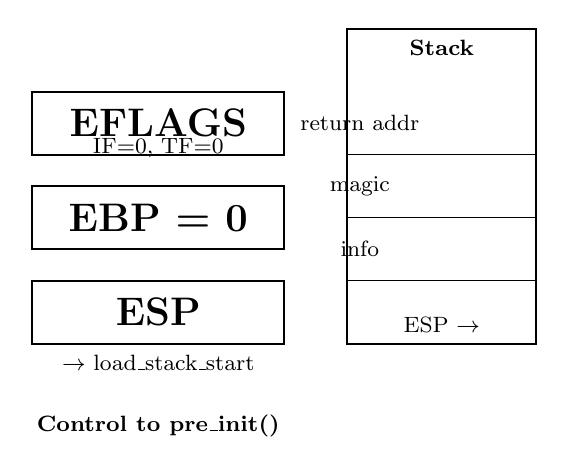
\begin{tikzpicture}[scale=0.8]
  % CPU registers
  \draw[thick] (0,0) rectangle (4,1);
  \node at (2, 0.5) [font=\Large\bfseries] {ESP};
  \node at (2, -0.3) [font=\footnotesize] {$\rightarrow$ load\_stack\_start};

  \draw[thick] (0,1.5) rectangle (4,2.5);
  \node at (2, 2) [font=\Large\bfseries] {EBP = 0};

  \draw[thick] (0,3) rectangle (4,4);
  \node at (2, 3.5) [font=\Large\bfseries] {EFLAGS};
  \node at (2, 3.1) [font=\footnotesize] {IF=0, TF=0};

  % Stack diagram
  \draw[thick] (5,0) rectangle (8,5);
  \node at (6.5, 4.7) [font=\footnotesize\bfseries] {Stack};
  \draw (5,3) -- (8,3); \node at (5.2, 3.5) [font=\footnotesize] {return addr};
  \draw (5,2) -- (8,2); \node at (5.2, 2.5) [font=\footnotesize] {magic};
  \draw (5,1) -- (8,1); \node at (5.2, 1.5) [font=\footnotesize] {info};
  \node at (6.5, 0.3) [font=\footnotesize] {ESP $\rightarrow$};

  \path[thick,->] (2, -0.5) -- (2, -1);
  \node at (2, -1.3) [font=\footnotesize\bfseries] {Control to pre\_init()};
\end{tikzpicture}
\caption{CPU State at pre\_init() Entry}
\label{fig:cpu-state-at-entry}
\end{figure}

\section{Summary: Entry Point Responsibilities}

\begin{enumerate}
\item \textbf{Bootloader Interface}: Confirm Multiboot contract and extract info
\item \textbf{Stack Setup}: Establish kernel stack before C execution
\item \textbf{CPU State Initialization}: Set flags to known good state
\item \textbf{C Environment Preparation}: Zero frame pointer, align stack
\item \textbf{Parameter Passing}: Push bootloader info as function arguments
\item \textbf{Control Transfer}: Jump to pre\_init() C function
\end{enumerate}

The next chapter continues the trace into pre\_init() and toward kmain().
